\documentclass{beamer}
\usepackage[utf8]{inputenc}
\usepackage{graphicx}

\newtheorem{definicion}{Definición}
\newtheorem{ejemplo}{Ejemplo}
\title[Método de Bisección]{Metodo de Bisección}
\author[Equipo 1 G]{Equipo 1-G}
\date[11-05-2014]{11 de mayo de 2014}
\usetheme{Madrid}

%%%%%%%%%%%%%%%%%%%%%%%%%%%%%%%%%%%%%%%%%%%%%%%%%%%%%%%%%%%%%%%%%%%%%%%%%%%%%%%

\begin{document}
  
%++++++++++++++++++++++++++++++++++++++++++++++++++++++++++++++++++++++++++++++  

\begin{frame}

  \begin{small}
    \begin{center}
     Facultad de Matemáticas \\
     Universidad de La Laguna
    \end{center}
  \end{small}

\end{frame}

%++++++++++++++++++++++++++++++++++++++++++++++++++++++++++++++++++++++++++++++  
\begin{frame}
  \frametitle{Índice}  
  \tableofcontents[pausesections]
\end{frame}
%++++++++++++++++++++++++++++++++++++++++++++++++++++++++++++++++++++++++++++++  


\section{Motivación y objetivos}
\begin{frame}

\frametitle{Motivación y objetivos}
\begin{Motivation}
    Aplicar los conocimientos obtenido en python para resolver una función según el método de la bisección.
\end{Motivation}

\begin{Objetivos}
     Resolver, mediante el método de la bisección (usando python) la función sin(x).
\end{Objetivos}

\end{frame}
%++++++++++++++++++++++++++++++++++++++++++++++++++++++++++++++++++++++++++++++  

\section{Fundamentos teóricos}
\begin{frame}

\frametitle{Fundamentos teóricos}

\begin{block}{Explicación}
  \begin{itemize}
  \item
    Se basa en el Teorema del Valor Intermedio (TVI), el cual establece que toda función continua f en un intervalo cerrado [a,b] toma todos los valores que se hallan entre f(a) y f(b). 
  \pause

  \item
    Esto es que: todo valor entre f(a) y f(b) es la imagen de al menos un valor en el intervalo [a,b]. 
  \pause

  \item
    En caso de que f(a) y f(b) tengan signos opuestos, el valor cero sería un valor intermedio entre f(a) y f(b), por lo que con certeza existe un p en [a,b] que cumple f(p) = 0. 
  \pause

  \item
    De esta forma, se asegura la existencia de al menos una solución de la ecuación f(x) = 0.
  \end{itemize}
\end{block}

\end{frame}

%++++++++++++++++++++++++++++++++++++++++++++++++++++++++++++++++++++++++++++++  

\section{Procedimiento experimental}

\subsection{Procedimiento (Parte 1)}
\begin{frame}
\frametitle{Procedimiento}
El método de la bisección es un proceso iterativo que sigue los siguientes pasos:
 \item
  Se "parte" por la mitad el intervalo [a,b]. Por lo que se cogen los valores de los extremos y se dividen por $2$.
  \begin{center}
   $$ c_1=\frac{a+b}{2} $$
  \end{center}
 \pause
 
 \item
  Luego hay que mirar los signos de la función en el punto c y comparar con los signos de la función de los extremos.
    \Item
     Si $f(a)*f(c)<0$ se sustituye $c$ por $b$ quedandose $$c_2=\frac{a+c_1}{2}$$
    \Item
     Si $f(b)*f(c)<0$ se sustituye $c$ por $a$ quedandose $$c_2=\frac{c_1+b}{2}$$
\end{frame}

%++++++++++++++++++++++++++++++++++++++++++++++++++++++++++++++++++++++++++++++  

\subsection{Procedimiento (Parte 2)}
\begin{frame}
\frametitle{Procedimiento}

 \item
  Este proceso se va haciendo hasta que la función en el punto $c_n$ es igual a $0$
 \pause
 
 \item
  Hay que tener en cuenta que este método tiene un error y se puede calcular con:
  \begin{center}
   $$ error=\frac{b-a}{2^n} $$ 
  \end{center} 
  Siendo n las veces que se ha partido.
 
\end{frame}

%++++++++++++++++++++++++++++++++++++++++++++++++++++++++++++++++++++++++++++++  

\subsection{Código} 
\begin{frame}[fragile]

\frametitle{Código}
\begin{center}
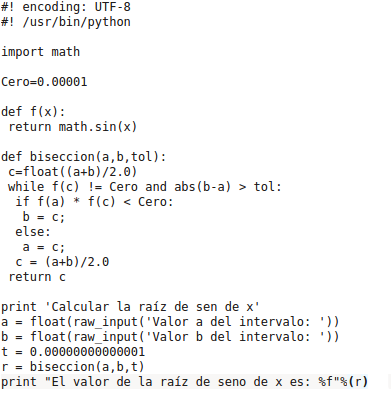
\includegraphics[width=0.6\textwidth]{xcgc.png} 
\end{center}
\end{frame}

%++++++++++++++++++++++++++++++++++++++++++++++++++++++++++++++++++++++++++++++  

\section{Conclusiones}
\begin{frame}[fragile]
\frametitle{Conclusiones}

\end{frame}


%++++++++++++++++++++++++++++++++++++++++++++++++++++++++++++++++++++++++++++++  

\section{Bibliografía}
\begin{frame}
  \frametitle{Bibliografía}

  \begin{thebibliography}{10}

    \beamertemplatebookbibitems
    \bibitem[Wikipedia]{wiki}  
    Método de bisección 
    {\small $http://es.wikipedia.org/wiki/M\'etodo\_de\_bisecci\'on$}

    \beamertemplatebookbibitems
    \bibitem[Campus Virtual, 2014]{guia}  
    Algoritmo de bisección.
    (2014) 
    {\small $PDF del aula virtual de la asignatura de Infórmatica$}
    
\beamertemplatebookbibitems
    \bibitem[Campus Virtual, 2014]{yt}  
    Algoritmo de bisección.
    (2014) 
    {\small $https://www.youtube.com/watch?v=dimOkJ6WZz0$}

  \end{thebibliography}
\end{frame}

%++++++++++++++++++++++++++++++++++++++++++++++++++++++++++++++++++++++++++++++  

\end{document}
